\documentclass[11pt,a4paper]{article}
\usepackage[T1]{fontenc}
\usepackage[utf8]{inputenc}
\usepackage{lmodern}
\usepackage[margin=24mm]{geometry}
\usepackage{amsmath,amssymb,amsthm,mathtools}
\usepackage{graphicx,booktabs,array,tabularx}
\usepackage{enumitem}
\usepackage{tikz}
\usepackage{xcolor}
\definecolor{plum}{HTML}{70365F}
\definecolor{teal}{HTML}{167C80}
\usepackage[colorlinks=true,linkcolor=plum,citecolor=teal,urlcolor=teal]{hyperref}
\usepackage{microtype}
\newtheorem{theorem}{Theorem}[section]
\newtheorem{proposition}[theorem]{Proposition}
\newtheorem{corollary}[theorem]{Corollary}
\newtheorem{lemma}[theorem]{Lemma}
\theoremstyle{definition}\newtheorem{conjecture}{Conjecture}
\newtheorem{definition}[theorem]{Definition}
\theoremstyle{remark}\newtheorem{remark}[theorem]{Remark}
\newcommand{\eps}{\varepsilon}
\newcommand{\R}{\mathbb{R}}
\newcommand{\dd}{\,\mathrm{d}}
\newcommand{\status}[1]{\textsf{\small #1}}
\setlist{itemsep=1pt,topsep=3pt}
\title{Backtracking-weighted PageRank is not coordinatewise monotone:\\
minimal counterexamples, a certified census and endpoint tests}
\author{Anonymous}
\date{23 October 2026\\[2pt]\small Version 1.0.0-candidate (unrefereed). DOI: \href{https://doi.org/10.5281/zenodo.23580381}{10.5281/zenodo.23580381}.\\
\small Code and data: \url{https://github.com/ipitchford/pagerank-backtracking-nonmonotone}}
\begin{document}
\maketitle

\begin{abstract}
\noindent\textbf{Plain-language summary.}
PageRank scores the vertices of a network by a random walk that occasionally restarts. A walk may be told to avoid stepping straight back along the edge it has just used (non-backtracking), to behave as usual, or to bounce back and forth. Glover, Jones, Kempton and Oveson conjectured that, as the return weight $\mu$ is turned up, every vertex score moves in one direction only. If true, two cheap calculations would tell an analyst which way the expensive non-backtracking score lies. We show that the conjecture is false, and that its failure is common rather than exotic.

\smallskip\noindent\textbf{Results.}
On the five-vertex house graph the roof vertex first loses and then regains score; an exact rational certificate proves this, and a closed cubic formula classifies every damping value. Among graphs of minimum degree two, five vertices is the smallest order for \emph{every} damping value: the house covers $\eps>\eps_c\approx0.2407$ and the gem covers $\eps\leq1/3$. If leaves are allowed, the four-vertex paw fails for small and for large damping, where four is then the smallest order; at intermediate damping it is five. Even a five-vertex tree fails. An exact census of all 995 connected graphs on two to seven vertices, at five damping values, finds a nonmonotone vertex in $675$ of the $853$ seven-vertex graphs. Both readings of the conjecture's spread clause also fail exactly, even when the extreme vertices are unique. We prove a two-step criterion that explains which vertices dip at small damping, and an exact formula for the slope at ordinary PageRank that gives cheap sufficient tests. Numerical experiments find that 10--41\% of the vertices of standard networks are nonmonotone; the excursions are small and rankings rarely change. We also characterise exact invariance under backtracking and refute the degree-tail Conjecture~3.2 of the same paper, in its local-weak-convergence reading, for every tail index above one. Every theorem is backed by an exact proof; every computational claim is labelled as exact or numerical.
\end{abstract}

\tableofcontents

\section{Introduction}
\subsection{The question}
PageRank combines movement along edges with occasional restart. A walk with memory can change the weight of an immediate return along the edge just used. The parameter $\mu\geq0$ gives that return weight $\mu$ and each alternative weight one. Thus $\mu=0$ forbids immediate returns, $\mu=1$ is ordinary PageRank, and $\mu\to\infty$ makes the walk oscillate on a single edge. Glover, Jones, Kempton and Oveson \cite{glover,gloverarxiv} studied the resulting vertex scores $\pi_\mu$ and stated two conjectures in Sections~3.3 and~3.4 of their paper. We quote them verbatim from arXiv:2211.13353v2 (9 February 2026). The journal version \cite{glover} was not accessible to us, so we could not compare its wording.

\begin{conjecture}[{\cite[Conjecture 3.1]{gloverarxiv}}]\label{conj:31}
``The function $(\pi_{\mu})_{i}$ is monotonic for all $i$ and
\[
  \max_{i}\pi_{\mu}(i)-\min_{i}\pi_{\mu}(i)\leq\max_{i}\pi_{\mu+\alpha}(i)-\min_{i}\pi_{\mu+\alpha}(i)
\]
for all $\alpha>0$.''
\end{conjecture}

\begin{conjecture}[{\cite[Conjecture 3.2]{gloverarxiv}}]\label{conj:32}
``If $d_{i}\sim X$ where $X$ is a regularly-varying random variable and $d_{i}$ is the degree of node $i\in V(G)$, then $\pi_{\infty}(i)$ will also be scale-free.''
\end{conjecture}

Conjecture~\ref{conj:31} is a conjunction of a \emph{coordinatewise clause} and a \emph{spread clause}. The coordinatewise clause is the substantive one. The source motivates it computationally: the infinite-backtracking score $\pi_\infty$ has a cheap closed form, so if each coordinate were monotone, comparing $\pi_\infty$ with ordinary PageRank $\pi_1$ would tell which side of $\pi_1$ the non-backtracking score $\pi_0$ lies on.

\subsection{A three-number certificate}
For the house graph (Figure~\ref{fig:house}) with uniform restart and damping $\eps=1/2$, the roof vertex has
\begin{equation}\label{eq:shortcertificate}
 \pi_0(4)=\frac{638}{3615},\qquad
 \pi_1(4)=\frac{22}{125},\qquad
 \pi_\infty(4)=\frac{8}{45},
\end{equation}
so that $\pi_0(4)-\pi_1(4)=44/90375>0$ and $\pi_\infty(4)-\pi_1(4)=2/1125>0$. Both endpoints lie strictly above the middle value, so the roof score is not monotone in $\mu$. Monotone interpolation would put the two endpoints on opposite sides of $\pi_1(4)$, so the proposed shortcut points the wrong way here.

\subsection{Roadmap and summary of results}
Section~\ref{sec:model} fixes the model, including leaves. Sections~\ref{sec:house}--\ref{sec:classification} give the exact house response and its damping classification. Section~\ref{sec:minimal} identifies the smallest counterexamples, with and without the minimum-degree assumption, and lifts them to arbitrarily large graphs. Section~\ref{sec:why} explains the dip and gives cheap tests. Section~\ref{sec:census} reports the certified census. Section~\ref{sec:spread} settles the spread clause. Section~\ref{sec:invariance} characterises exact invariance. Section~\ref{sec:prevalence} measures prevalence and practical impact numerically. Section~\ref{sec:tails} treats Conjecture~\ref{conj:32}. Section~\ref{sec:verification} describes the verification code, and Section~\ref{sec:conclusion} concludes. Table~\ref{tab:summary} lists the results. ``Proved'' means a complete mathematical proof in this paper (some steps are exact polynomial identities checked by the accompanying code). ``Certified'' means an exact computation: a finite exact certificate, or an exhaustive exact search where so stated. ``Numerical'' means floating-point evidence only.

\begin{table}[htbp]
\centering\small
\caption{Summary of results. Status: P = proved; C = certified exact computation; N = numerical. Novelty: ``new'' means not found within our literature search (Section~\ref{sec:verification}); ``inherited'' means taken from, or a direct adaptation of, the cited work.}\label{tab:summary}
\setlength{\tabcolsep}{4pt}\begin{tabularx}{\textwidth}{@{}>{\raggedright\arraybackslash}p{2.9cm}X>{\centering\arraybackslash}p{1.1cm}>{\raggedright\arraybackslash}p{1.9cm}@{}}
\toprule
Result & Content & Status & Novelty\\
\midrule
Thms \ref{thm:response}, \ref{thm:threshold} & House roof: cubic formula; monotone iff $\eps\leq\eps_c$; one minimum, at $\mu=1$ iff $\eps=4/9$ & P & new\\
Prop.~\ref{prop:shortcut} & Endpoint shortcut is wrong for the roof iff $\eps>\eps_0\approx0.3291$ & P & new\\
Thm~\ref{thm:minimal} & Min.\ degree $\geq2$: order 5 is minimal for \emph{every} $\eps$ (house $\cup$ gem) & P & new\\
Prop.~\ref{prop:paw}, Cor.~\ref{cor:nmin} & With leaves: the paw fails iff $\eps\in(0,\eps_1)\cup(\eps_2,1)$; minimal order is 4 there and 5 on $[\eps_1,\eps_2]$ & P & new\\
Prop.~\ref{prop:tree} & A five-vertex tree with a nonmonotone leaf on $(0,1)$ & C & new\\
Lemma~\ref{lem:cover}, Cor.~\ref{cor:family} & Failures lift through covers to every order $5k$ & P & lemma inherited \cite{boldifib}\\
Thm~\ref{thm:twostep} & Small-damping two-step criterion; sign test $\sigma_j$ & P & new\\
Prop.~\ref{prop:slope}, Cor.~\ref{cor:tests} & Exact slope at $\mu=1$; three endpoint tests & P & new\\
Section~\ref{sec:census} & Census of all connected graphs on $\leq7$ vertices, five $\eps$ & C & new\\
Prop.~\ref{prop:spread}, \ref{prop:uniquespread} & Spread clause fails as printed and when reversed, also with unique extreme vertices & P, C & new\\
Thm~\ref{thm:invariance} & Exact invariance iff $P^2v=v$ & P & converse new; sufficiency \cite{arrigo,glover}\\
Section~\ref{sec:prevalence} & Prevalence, dip sizes, shortcut failures, rank stability & N & new\\
Prop.~\ref{prop:reversal} & An exact transient rank reversal (Les Mis\'erables) & C & new\\
Thm~\ref{thm:tails} & Conjecture~\ref{conj:32} fails for every tail index $\alpha>1$ & P & mechanism inherited \cite{henning}\\
Prop.~\ref{prop:degreebound} & $n\pi_\infty(i)\leq(1+\eps d_i/2)/(1+\eps)$ & P & elementary\\
\bottomrule
\end{tabularx}
\end{table}

\section{The model}\label{sec:model}
Let $G=(V,E)$ be a finite connected simple undirected graph with degrees $d_i$, and let $\vec E$ be the set of the two orientations of each edge. A state $(i,j)\in\vec E$ records the directed edge last used; we call $i$ its \emph{tail}. For $\mu\geq0$ define the column-stochastic matrix $Q_\mu$ by
\begin{equation}\label{eq:kernel}
 (Q_\mu)_{(j,k),(i,j)}=
 \frac{1+(\mu-1)\mathbf{1}_{\{k=i\}}}{d_j-1+\mu}
 \quad(k\sim j),
\end{equation}
with all other entries zero. If $d_j\geq2$, the denominator satisfies $d_j-1+\mu\geq1$.

\emph{Leaves.} If $d_j=1$, the only continuation is the return, and \eqref{eq:kernel} gives it weight $\mu/\mu=1$ for every $\mu>0$. At $\mu=0$ the source's kernel is undefined at a leaf, because the corresponding entry of $\hat D-I$ vanishes. We use the same forced return at $\mu=0$, which is the limit $\mu\to0^+$, that is, the continuous extension of the source kernel; this endpoint choice is ours. For $\mu>0$ the kernel agrees with node2vec with return parameter $p=1/\mu$ and in--out parameter $q=1$ \cite{grover,meng}. It differs from some of the leaf conventions of Aleja et al.\ \cite{aleja}. Every nonmonotonicity statement we make on a graph with leaves concerns the open range $\mu\in(0,\infty)$, where no convention is needed. For graphs of minimum degree at least two, which is the setting of the source's theorems, the kernel needs no convention at any $\mu\geq0$.

Let $v$ be a probability vector on $V$, spread restart mass evenly over outgoing edges, $u_{ij}=v_i/d_i$, and fix a damping (follow) probability $0<\eps<1$. The edge PageRank and vertex scores are
\begin{equation}\label{eq:balance}
 q_\mu=(1-\eps)u+\eps Q_\mu q_\mu,
 \qquad
 \pi_\mu(i)=\sum_{j\sim i}q_\mu(i,j).
\end{equation}
Since $\|\eps Q_\mu\|_1=\eps<1$, the solution $q_\mu=(1-\eps)\sum_{t\geq0}\eps^tQ_\mu^tu$ is unique, nonnegative and of total mass one. For uniform restart $v_i=1/n$ we say \emph{uniform restart}. It is used throughout unless stated otherwise.

\begin{remark}[Faithfulness and projection]\label{rem:faithful}
In the notation of \cite[Definition~2.4]{gloverarxiv}, $Q_\mu=C_\mu^T(\hat D-(1-\mu)I)^{-1}$, $u=T^T(TT^T)^{-1}v$ and $\pi_\mu=T\hat\pi_\mu$; this is the tail projection. (The source writes $H_\mu^T\hat y=\hat y$ in some proofs, which is inconsistent with the column-stochastic $H_\mu$ of its Definition~2.4. We use the column-stochastic reading.) The head projection $H_\mu(j)=\sum_iq_\mu(i,j)$ satisfies $\pi_\mu=(1-\eps)v+\eps H_\mu$, because every state leaving $j$ is entered either by restart at $j$ or from a state with head $j$. Hence monotonicity of a coordinate does not depend on which projection is used. On $\mu\in[0,1]$ the model is the unweighted, leaf-free special case of \cite[Definitions 3.5, 3.7]{aleja}. Related formulations are \cite{arrigo,criado,zhang}. It is a first-order memory (edge-lift, Hashimoto \cite{hashimoto}) model; it should not be confused with multilinear or second-order PageRank \cite{gleichlimyu,benson}, whose fixed point is nonlinear at the vertex level.
\end{remark}

The two endpoints have closed forms. With $A_G$ the adjacency matrix, $D_G=\operatorname{diag}(d_i)$ and $P=A_GD_G^{-1}$,
\begin{equation}\label{eq:endpoints}
 \pi_1=(1-\eps)(I-\eps P)^{-1}v,
 \qquad
 \pi_\infty=\frac{v+\eps Pv}{1+\eps}.
\end{equation}
The second identity is \cite[Proposition 3.3]{gloverarxiv}. At $\mu=1$ one also has $q_1(i,j)=\pi_1(i)/d_i$.

\section{An exact response on the house graph}\label{sec:house}
Use vertices $0,\dots,4$ and edges
\begin{equation}\label{eq:houseedges}
 E=\{01,03,04,12,14,23\}.
\end{equation}
Vertices 0 and 1 have degree three; vertices 2, 3 and the roof 4 have degree two.

\begin{figure}[htbp]
\centering
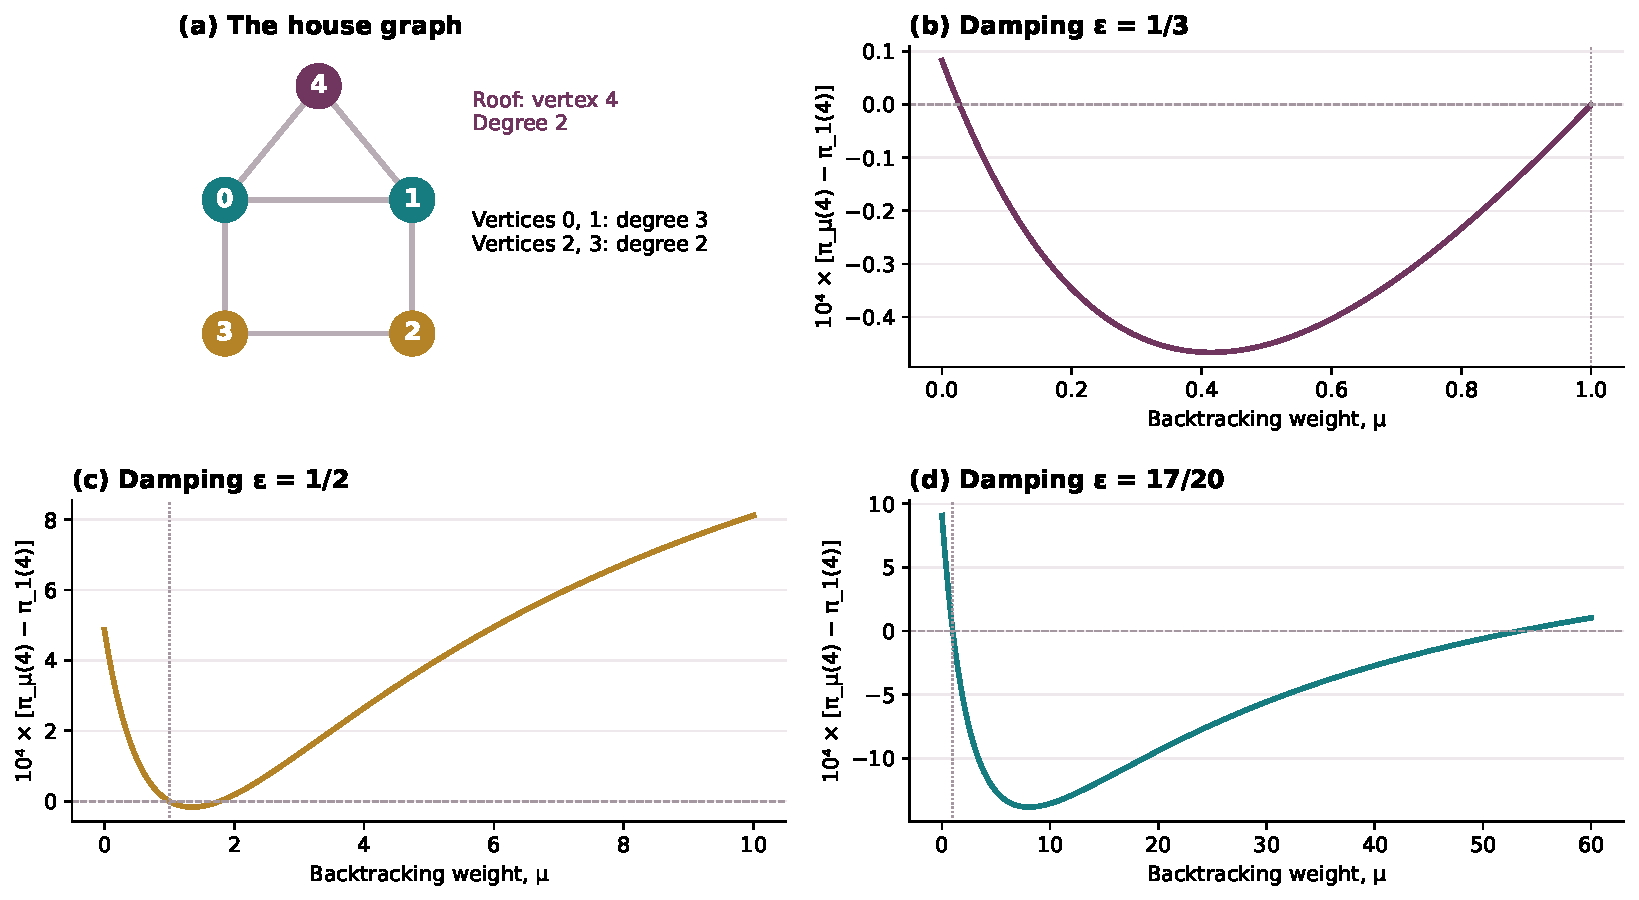
\includegraphics[width=\textwidth]{house_response.pdf}
\caption{(a) The house graph. (b)--(d) The exact roof response \eqref{eq:response}, plotted as $10^4[\pi_\mu(4)-\pi_1(4)]$ for $\eps=1/3$ on $\mu\in[0,1]$, $\eps=1/2$ on $[0,10]$ and $\eps=17/20$ on $[0,60]$. In (b) the minimum lies inside $[0,1]$ because $\eps<4/9$. The curves illustrate the theorems; they are not part of any proof.}\label{fig:house}
\end{figure}

\begin{theorem}[Cubic roof response]\label{thm:response}
Put $s=(1-\eps)\mu$. For the house graph with uniform restart,
\begin{equation}\label{eq:response}
 \pi_\mu(4)=\frac{N_\eps(s)}{15D_\eps(s)},\qquad
 N_\eps(s)=\sum_{j=0}^3 n_js^j,\quad
 D_\eps(s)=\sum_{j=0}^3 d_js^j,
\end{equation}
with the coefficients in Table~\ref{tab:coeff}. In particular $D_\eps(s)>0$ for $s\geq0$. At $\eps=1/2$,
$\pi_\mu(4)=2(12\mu^3+115\mu^2+346\mu+319)/[15(9\mu^3+87\mu^2+263\mu+241)]$.
\end{theorem}

\begin{table}[htbp]
\centering\small
\caption{Coefficients of the roof response \eqref{eq:response}. The variable $s=(1-\eps)\mu$ makes every coefficient a polynomial in $\eps$ with positive coefficients.}\label{tab:coeff}
\begin{tabular}{@{}cll@{}}
\toprule
$j$ & $n_j$ & $d_j$\\
\midrule
0 & $2\eps^5+4\eps^4+9\eps^3+10\eps^2+8\eps+12$ & $\eps^5+2\eps^4+3\eps^3+4\eps^2+4\eps+4$\\
1 & $6\eps^4+13\eps^3+25\eps^2+22\eps+24$ & $3\eps^4+6\eps^3+10\eps^2+10\eps+8$\\
2 & $6\eps^3+14\eps^2+19\eps+15$ & $3\eps^3+6\eps^2+8\eps+5$\\
3 & $(1+\eps)(3+2\eps)$ & $(1+\eps)^2$\\
\bottomrule
\end{tabular}
\end{table}

\begin{proof}
The automorphism exchanging $0\leftrightarrow1$ and $2\leftrightarrow3$ preserves the kernel and the restart, so by uniqueness the edge masses are constant on its six orbits:
\[
 a=q_{01}=q_{10},\ b=q_{03}=q_{12},\ c=q_{30}=q_{21},\ d=q_{23}=q_{32},\ h=q_{04}=q_{14},\ f=q_{40}=q_{41}.
\]
Write $r=\mu+2$, $w=\mu+1$, $t_A=(1-\eps)/15$ and $t_B=(1-\eps)/10$. After multiplying each balance equation by its denominator $d_j-1+\mu$, the equations become
\begin{equation}\label{eq:quotient}
\begin{aligned}
 (r-\eps\mu)a-\eps c-\eps f&=rt_A, &
 -\eps a+rb-\eps\mu c-\eps f&=rt_A,\\
 -\eps\mu b+wc-\eps d&=wt_B, &
 -\eps b+(w-\eps\mu)d&=wt_B,\\
 -\eps a-\eps c+rh-\eps\mu f&=rt_A, &
 -\eps h+f&=t_B.
\end{aligned}
\end{equation}
In the last equation the two incoming masses at the roof are equal, so the ordinary and return weights combine to $w$. The roof score is $2f$. Let $M$ be the coefficient matrix in the order $(a,b,c,d,h,f)$ and $b_{30}=30(rt_A,rt_A,wt_B,wt_B,rt_A,t_B)^T$. Expansion gives the polynomial identities
\[
 \det M=(\mu+1)(\mu+2)(1-\eps)D_\eps(s),\qquad
 \det M[f\leftarrow b_{30}]=(\mu+1)(\mu+2)(1-\eps)N_\eps(s),
\]
which the code checks coefficient by coefficient over $\mathbb Q[\mu,\eps]$. Cramer's rule gives $f=N_\eps/(30D_\eps)$.
\end{proof}

\section{The complete damping classification of the roof vertex}\label{sec:classification}
\begin{theorem}[One threshold, one minimum]\label{thm:threshold}
Let $\eps_c$ be the unique root in $(0,1/4)$ of
\begin{equation}\label{eq:A}
 A(\eps)=\eps^6-2\eps^5-9\eps^4-11\eps^3-16\eps^2-12\eps+4,
\end{equation}
so that $2406813\cdot10^{-7}<\eps_c<2406814\cdot10^{-7}$. For the house roof:
\begin{enumerate}
 \item if $0<\eps\leq\eps_c$, then $\pi_\mu(4)$ is strictly increasing on $[0,\infty)$;
 \item if $\eps_c<\eps<1$, then $\pi_\mu(4)$ decreases to exactly one strict minimum at some $\mu_*(\eps)>0$ and then increases;
 \item for $\eps>\eps_c$, the minimum lies below, at or above $\mu=1$ according as $\eps<4/9$, $\eps=4/9$ or $\eps>4/9$. Since $\eps_c<4/9$, each case occurs.
\end{enumerate}
\end{theorem}

\begin{proof}
Let $B(\eps)=4\eps^5-4\eps^4-14\eps^3-18\eps^2-16\eps+12$, $C(\eps)=6\eps^4-\eps+13$ and
\[
 R_\eps(s)=(1+\eps)^2s^4+2(1+\eps)(2\eps^2+3)s^3+C(\eps)s^2+B(\eps)s+A(\eps).
\]
Differentiating \eqref{eq:response} gives the polynomial identity
\begin{equation}\label{eq:derivative}
 \frac{\dd}{\dd\mu}\pi_\mu(4)=\frac{\eps^2(1-\eps)R_\eps(s)}{15D_\eps(s)^2}.
\end{equation}
The three leading coefficients of $R_\eps$ are positive, since $C(\eps)>12$. On $(0,1)$ we have $A'(\eps)=6\eps^5-10\eps^4-36\eps^3-33\eps^2-32\eps-12<0$, because $6\eps^5\leq6\eps^4<10\eps^4$. Also $A(0)=4$ and $A(1/4)<0$, so $A$ has one root $\eps_c$ in $(0,1/4)$ and is negative on $(\eps_c,1)$. Exact substitution gives the bracket. For $0<\eps\leq1/4$,
$B(\eps)\geq12-16/4-18/16-14/64-4/256>0$. Hence, if $\eps\leq\eps_c$, all coefficients of $R_\eps$ are nonnegative and only the constant one can vanish, and $\pi_\mu(4)$ is strictly increasing. If $\eps>\eps_c$, the constant coefficient is negative and the three leading ones are positive, so the coefficient sequence has exactly one sign change whatever the sign of $B$. By Descartes' rule there is exactly one positive root, and it is simple. The derivative changes from negative to positive there. Finally, $[(\partial_\mu N)D-N(\partial_\mu D)]_{\mu=1}=9\eps^2(1-\eps)(4-9\eps)$ with $N=N_\eps((1-\eps)\mu)$ and $D=D_\eps((1-\eps)\mu)$, which locates the minimum relative to $\mu=1$.
\end{proof}

\begin{corollary}[Failure inside the original range]\label{cor:unit}
Monotonicity fails even for $\mu$ restricted to $[0,1]$: at $\eps=1/3$,
$\pi_0(4)=3929/21570$, $\pi_{1/2}(4)=1481/8133$ and $\pi_1(4)=51/280$, and the middle value is strictly the smallest.
\end{corollary}

\begin{proposition}[Exact failure range of the endpoint shortcut]\label{prop:shortcut}
Let $\eps_0$ be the unique root in $(0,1)$ of $F(\eps)=2\eps^4+\eps^3+6\eps^2+10\eps-4$, so that $3291037\cdot10^{-7}<\eps_0<3291038\cdot10^{-7}$. For every $\eps$, $\pi_\infty(4)>\pi_1(4)$. Moreover $\pi_0(4)>\pi_1(4)$ precisely when $\eps>\eps_0$.
\end{proposition}
\begin{proof}
One has $\pi_1(4)=(6-\eps)/[5(6+\eps-\eps^2)]$ and $\pi_\infty(4)=(3+2\eps)/[15(1+\eps)]$, so
\[
 \pi_\infty(4)-\pi_1(4)=\frac{2\eps^2(1-\eps)}{15(1+\eps)(6+\eps-\eps^2)}>0,\qquad
 \pi_0(4)-\pi_1(4)=\frac{\eps^2(1-\eps)F(\eps)}{15d_0(6+\eps-\eps^2)}.
\]
Since $F(0)<0<F(1)$ and $F'>0$, the zero is unique.
\end{proof}

\begin{remark}[Two different thresholds]
For $\eps_c<\eps\leq\eps_0$ the roof is nonmonotone, yet the shortcut still gives the right side for $\pi_0$, because the minimum is shallow at $\mu=0$. The directional error needs $\eps>\eps_0$. It includes the conventional damping $\eps=17/20$, where $\pi_0(4)=12276466/72640495$, $\pi_1(4)=412/2451$ and $\pi_\infty(4)=94/555$.
\end{remark}

\section{Smallest counterexamples and large examples}\label{sec:minimal}
Two further graphs appear (Figure~\ref{fig:small}). The \emph{gem} is the path $0$--$1$--$2$--$3$ together with an apex $4$ adjacent to all four path vertices. The \emph{paw} is a triangle $1,2,3$ with a pendant vertex $0$ attached at $3$.

\begin{figure}[htbp]
\centering
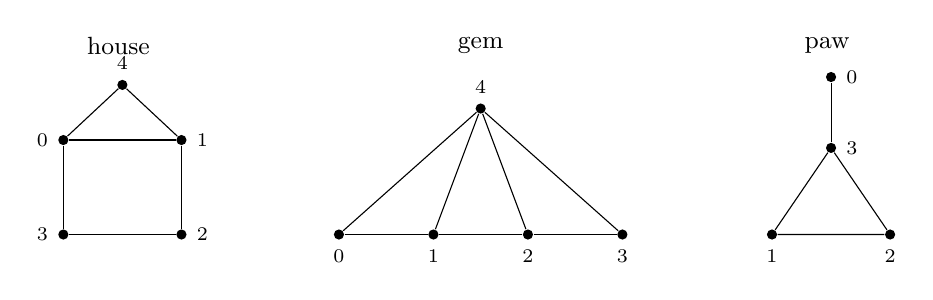
\begin{tikzpicture}[x=1mm,y=1mm,every node/.style={font=\scriptsize},v/.style={circle,fill=black,inner sep=1.3pt}]
\node at (12,28) {\small house};
\node[v,label=left:0] (h0) at (5,16) {}; \node[v,label=right:1] (h1) at (20,16) {};
\node[v,label=right:2] (h2) at (20,4) {}; \node[v,label=left:3] (h3) at (5,4) {};
\node[v,label=above:4] (h4) at (12.5,23) {};
\draw (h0)--(h1)--(h2)--(h3)--(h0); \draw (h0)--(h4)--(h1);
\node at (58,28) {\small gem};
\node[v,label=below:0] (g0) at (40,4) {}; \node[v,label=below:1] (g1) at (52,4) {};
\node[v,label=below:2] (g2) at (64,4) {}; \node[v,label=below:3] (g3) at (76,4) {};
\node[v,label=above:4] (g4) at (58,20) {};
\draw (g0)--(g1)--(g2)--(g3); \foreach \x in {g0,g1,g2,g3} \draw (g4)--(\x);
\node at (102,28) {\small paw};
\node[v,label=below:1] (p1) at (95,4) {}; \node[v,label=below:2] (p2) at (110,4) {};
\node[v,label=right:3] (p3) at (102.5,15) {}; \node[v,label=right:0] (p0) at (102.5,24) {};
\draw (p1)--(p2)--(p3)--(p1); \draw (p3)--(p0);
\end{tikzpicture}
\caption{The house, the gem and the paw, labelled as in the text and the code.}\label{fig:small}
\end{figure}

\begin{proposition}[The gem fails at small damping]\label{prop:gem}
For the gem with uniform restart, write $\frac{\dd}{\dd\mu}\pi_\mu(1)=\eps^2(\eps-1)R(\mu,\eps)/S(\mu,\eps)$ with $S>0$ the square of the score denominator. Then $R$ has degree six in $\mu$ with leading coefficient $4(1-\eps^2)^4$,
\[
 R(\mu,0)=(\mu+2)^2(4\mu^4+22\mu^3+37\mu^2+12\mu-11),
\]
\[
 R(0,\eps)=4\eps^8+8\eps^7-16\eps^6-40\eps^5-15\eps^4+63\eps^3+148\eps^2+64\eps-44 .
\]
The polynomial $R(0,\cdot)$ is negative on $(0,\eps_g)$, where $\eps_g\in(0.3565987,0.3565988)$ is its first positive root. Consequently, for every $0<\eps<\eps_g$, the score $\pi_\mu(1)=\pi_\mu(2)$ increases at $\mu=0$ and decreases for all large $\mu$, so it is nonmonotone.
\end{proposition}
\begin{proof}
The scores are obtained by exact LU solution of the 14-state system over $\mathbb Q(\mu,\eps)$. The displayed polynomials, the positivity of $S$ (a square times a positive constant), and the absence of roots of $R(0,\cdot)$ in $(0,0.3565987)$ are certified by exact Sturm root counts (Section~\ref{sec:verification}). If $R(0,\eps)<0$, the derivative is positive at $\mu=0$. The leading coefficient is positive for $\eps<1$, so $R(\mu,\eps)>0$ and the derivative is negative for all large $\mu$. Exact witnesses: at $\eps=1/10$, the values $\pi_\mu(1)$ at $\mu=0,1/3,1$ are $53729499/266457580$, $4997753/24784610$ and $123/610$, and the middle one is strictly the largest. At $\eps=1/4$, the values at $\mu=0,1/10,1$ are $263957/1293580$, $263643/1292020$ and $51/250$.
\end{proof}

\begin{theorem}[Smallest order, for every damping]\label{thm:minimal}
For every fixed $\eps\in(0,1)$, five is the smallest order of a connected simple graph with minimum degree at least two on which some coordinate of $\pi_\mu$ (uniform restart) is nonmonotone in $\mu\in[0,\infty)$. A witness is the gem when $\eps\leq1/3$ and the house when $\eps>\eps_c$.
\end{theorem}
\begin{proof}
Since $\eps_c<1/4<1/3<\eps_g$, Proposition~\ref{prop:gem} and Theorem~\ref{thm:threshold} cover every $\eps$. At order three the only eligible graph is $K_3$. At order four the complement has maximum degree one, so the eligible graphs are $C_4$, $K_4$ and the diamond $K_4-e$. Regular graphs have $\mu$-independent scores (Theorem~\ref{thm:invariance}). In the diamond (hubs $0,1$, tips $2,3$), let $a$, $b$, $c$ be the hub-to-hub, hub-to-tip and tip-to-hub masses. With $r=\mu+2$, the orbit balances
\[
 (r-\eps\mu)a-2\eps c=\tfrac{r(1-\eps)}{12},\quad
 -\eps a+rb-\eps(\mu+1)c=\tfrac{r(1-\eps)}{12},\quad
 -\eps b+c=\tfrac{1-\eps}{8}
\]
give the tip score
\[
 z_\mu=2c=\frac{(3-\eps-2\eps^2)\mu+2\eps^2+4\eps+6}{12[(1-\eps^2)\mu+\eps^2+2\eps+2]},
 \qquad
 z_\mu'=\frac{\eps^2(1-\eps)}{12[(1-\eps^2)\mu+\eps^2+2\eps+2]^2}>0,
\]
and the hub scores equal $1/2-z_\mu$. Every coordinate is therefore strictly monotone.
\end{proof}

\begin{proposition}[Leaves allowed: the paw is a smallest counterexample]\label{prop:paw}
With leaves allowed (Section~\ref{sec:model}), every coordinate is independent of $\mu$ on $K_2$, $K_3$ and the path $P_3$ (for $P_3$, $\pi=((2+\eps),2(1+2\eps),(2+\eps))/(6(1+\eps))$). On the paw with uniform restart, every coordinate has a derivative in $\mu$ whose numerator is a quadratic $a_2\mu^2+a_1\mu+a_0$ (times $\eps^2(1-\eps)$) with $a_2,a_1$ of one fixed sign on $(0,1)$. Let $\eps_1\in(0.0783254,0.0783255)$ be the root in $(0,1)$ of $2\eps^4+10\eps^3+9\eps^2+12\eps-1$, and $\eps_2\in(0.4355202,0.4355203)$ the root in $(0,1)$ of $\eps^4-6\eps^3+2\eps^2-9\eps+4$. Then:
\begin{enumerate}
 \item the leaf $0$ is monotone for every $\eps$;
 \item the degree-two vertices $1,2$ are nonmonotone exactly when $\eps<\eps_1$;
 \item the hub $3$ is nonmonotone exactly when $\eps>\eps_2$.
\end{enumerate}
Thus, without the degree restriction, order four is the smallest order with a nonmonotone coordinate for $\eps\in(0,\eps_1)\cup(\eps_2,1)$ (Corollary~\ref{cor:nmin}). At $\eps=1/2$ the hub values at $\mu=1/10,1/2,1$ are $2148/6389$, $344/1023$ and $39/116$, an interior maximum inside $(0,1]$.
\end{proposition}
\begin{proof}
$P_3$ is bipartite with parts of constant degree, and the displayed scores follow from the exact solve. For the paw, the coefficients are listed in the results file. In each case $a_2$ and $a_1$ share a constant sign on $(0,1)$, certified by exact Sturm root counts. The quadratic then has a positive root, necessarily simple, if and only if $a_0$ has the opposite sign, by Descartes' rule. The leaf's $a_0$ has the sign of $a_2$. For vertices 1 and 3, $a_0$ changes sign exactly once in $(0,1)$, at $\eps_1$ and $\eps_2$ respectively, with the stated orientation.
\end{proof}

\begin{corollary}[Smallest order with leaves allowed]\label{cor:nmin}
Let $n_{\min}(\eps)$ be the smallest order of a connected simple graph with a coordinate of $\pi_\mu$ (uniform restart) nonmonotone in $\mu\in(0,\infty)$. Then $n_{\min}(\eps)=4$ for $0<\eps<\eps_1$ and for $\eps_2<\eps<1$, and $n_{\min}(\eps)=5$ for $\eps_1\leq\eps\leq\eps_2$. With minimum degree at least two the smallest order is five for every $\eps$ (Theorem~\ref{thm:minimal}).
\end{corollary}
\begin{proof}
Orders two and three are $\mu$-independent by Proposition~\ref{prop:paw}. The connected graphs of order four are the star $K_{1,3}$, $C_4$, $K_4$, the diamond, the path $P_4$ and the paw. The star is bipartite biregular and $C_4$, $K_4$ are regular, so their scores do not depend on $\mu$ (exact symbolic solves; for $K_{1,3}$ the argument of Theorem~\ref{thm:invariance}(iv)$\Rightarrow$(i) applies verbatim, since a leaf returns with probability one). The diamond is monotone by the proof of Theorem~\ref{thm:minimal}. For $P_4$ (path $0$--$1$--$2$--$3$) the exact solve over $\mathbb Q(\mu,\eps)$ gives
\[
 \frac{\dd}{\dd\mu}\pi_\mu(0)=\frac{\dd}{\dd\mu}\pi_\mu(3)=-\frac{\dd}{\dd\mu}\pi_\mu(1)=-\frac{\dd}{\dd\mu}\pi_\mu(2)=\frac{\eps^2(1-\eps)}{8[(\eps^2-1)\mu-\eps^2-\eps-1]^2}>0,
\]
so every coordinate is strictly monotone. Only the paw remains, and Proposition~\ref{prop:paw} gives its exact failure set. Order five suffices for every $\eps$ by Theorem~\ref{thm:minimal}.
\end{proof}
The house and the gem cover overlapping damping ranges; no single five-vertex graph is claimed to fail at every $\eps$.

\begin{proposition}[A tree with a nonmonotone leaf]\label{prop:tree}
Take the tree with edges $04,13,23,34$, uniform restart and $\eps=1/2$. Its leaf $1$ has
\[
 \pi_\mu(1)=\frac{21\mu^2+95\mu+84}{15(9\mu^2+42\mu+37)},\qquad
 \frac{\dd}{\dd\mu}\pi_\mu(1)=\frac{27\mu^2+42\mu-13}{15(9\mu^2+42\mu+37)^2},
\]
so $\pi_\mu(1)$ decreases to a strict minimum at $\mu=(2\sqrt{22}-7)/9\approx0.2645$ and then increases. An exact certificate inside $(0,1)$: $\pi_{1/10}(1)=9371/61935$, $\pi_{1/4}(1)=349/2307$ and $\pi_{1/2}(1)=547/3615$, with successive differences $-398/15876005$ and $98/2779935$.
\end{proposition}
\begin{proof}
The rational response is the interpolated one of Section~\ref{sec:census}; the code checks the displayed closed form as a polynomial identity against it, and the three values by independent full eight-state solves. No convention at $\mu=0$ is involved.
\end{proof}

\begin{lemma}[Lifting through a finite cover]\label{lem:cover}
Let $\widetilde G$ be a $k$-sheeted cover of $G$, and lift the restart by assigning $v_i/k$ to each vertex over $i$. Then the lifted edge and vertex masses are $q_\mu(i,j)/k$ and $\pi_\mu(i)/k$ on every lift.
\end{lemma}
\begin{proof}
A covering map is a bijection on each neighbourhood. It therefore preserves degrees, the unique return, and the weights \eqref{eq:kernel}. The proposed masses satisfy every lifted balance equation and sum to one; uniqueness concludes. This is an instance of PageRank invariance under graph fibrations \cite{boldifib} (lumpability \cite{kemenysnell}) applied to the edge chain.
\end{proof}

\begin{corollary}[A positive fraction of failing vertices]\label{cor:family}
For every $k\geq2$ there is a connected simple graph on $5k$ vertices, with degrees two and three, in which $k$ vertices have $1/k$ times the house roof response. Their normalised scores $5k\,\pi_\mu$ equal $5\pi_\mu(4)$. In particular one fifth of the vertices are nonmonotone whenever $\eps>\eps_c$. Covers of the gem give graphs on $5k$ vertices, with degrees two, three and four, in which at least two fifths of the vertices (the lifts of gem vertices $1$ and $2$) are nonmonotone for $\eps<\eps_g$.
\end{corollary}
\begin{proof}
Take vertices $(i,t)$, $t\in\mathbb Z/k$. Lift every house edge within its sheet, except that $01$ becomes $(0,t)(1,t+1)$. Removing $01$ leaves the house connected, so each sheet is connected, and the shifted edges join consecutive sheets. Apply Lemma~\ref{lem:cover}. For the gem, shift the edge $01$ in the same way; removing it leaves the gem connected.
\end{proof}

\section{Why vertices dip, and cheap tests}\label{sec:why}
\subsection{A two-step picture}
Expand $q_\mu=(1-\eps)\sum_t\eps^tQ_\mu^tu$. The tail of a state after $t$ steps is distributed as $p_t(\cdot;\mu)$, where $p_0=v$ and $p_1=Pv$. Neither depends on $\mu$, because the first move out of the restart edge is uniform. The first $\mu$-dependence appears at $t=2$: the walk has moved $i\to j$ and now chooses between returning to $i$ and moving on. Under uniform restart, the mass arriving at $k$ after two steps is $p_2(k;\mu)=f_k(\mu)/n$, where
\begin{equation}\label{eq:twostep}
 f_k(\mu)=\sum_{j\sim k}\frac{d_kh_j-1+\mu}{d_k(d_j-1+\mu)},
 \qquad h_j=\sum_{l\sim j}\frac1{d_l}.
\end{equation}
Each term is a M\"obius function of $\mu$, increasing or decreasing according to the sign of
\[
 \sigma_j=\frac{d_j}{d_k}-h_j.
\]
So raising $\mu$ sends more two-step mass back to $k$ from a neighbour $j$ when $j$'s other neighbours have high degree (small $h_j$), and less when they have low degree. When the neighbours of $k$ disagree in sign, and their poles $d_j-1$ differ, the two-step profile can rise and then fall. That is the gem mechanism.

\begin{theorem}[Small-damping criterion]\label{thm:twostep}
Assume uniform restart and minimum degree at least two. Suppose $0\leq a<b<c$ and $\delta=f_k(b)-\max\{f_k(a),f_k(c)\}>0$ (respectively $\delta=\min\{f_k(a),f_k(c)\}-f_k(b)>0$). Then $\pi_\mu(k)$ is nonmonotone in $\mu$ for every $0<\eps<\delta/(n+\delta)$. If all $\sigma_j$, $j\sim k$, have the same weak sign, then $f_k$ is monotone, and any nonmonotonicity of $\pi_\mu(k)$ is a phenomenon of order $\eps^3$ or higher.
\end{theorem}
\begin{proof}
We have $\pi_\mu(k)=(1-\eps)[v_k+\eps(Pv)_k+\eps^2f_k(\mu)/n]+\rho_\mu$ with $0\leq\rho_\mu=(1-\eps)\sum_{t\geq3}\eps^tp_t(k;\mu)\leq\eps^3$. Hence $\pi_b(k)-\pi_a(k)\geq(1-\eps)\eps^2\delta/n-\eps^3>0$ when $(1-\eps)\delta>n\eps$, that is, $\eps<\delta/(n+\delta)$, and similarly for $c$. The function $(\alpha+\mu)/(\gamma+\mu)$ has derivative of the sign of $\gamma-\alpha$; here $\gamma-\alpha=d_j-d_kh_j=d_k\sigma_j$.
\end{proof}

\emph{The roof.} Both neighbours of the house roof have $\sigma=3/2-4/3=1/6>0$, so its two-step profile is increasing. The roof's dip is a third-order effect, which is why it needs damping above $\eps_c$. Heuristically, only longer walks see the competition between the shortcut $0$--$1$ (avoided when returns are suppressed) and the path $1$--$2$--$3$--$0$ (whose degree-two vertices funnel non-backtracking walkers forward). For gem vertex 1 the three neighbours give $\sigma=1/12,-1/12,-1/3$, and the dip already appears at second order. In the census (Section~\ref{sec:census}), $276$ of the $3985$ vertices of minimum-degree-two graphs have a nonmonotone two-step profile; $226$ of these are nonmonotone at $\eps=1/10$, out of $256$ such vertices in all. No vertex with uniform $\sigma$ signs has a nonmonotone profile, as the theorem predicts.

\subsection{The slope at ordinary PageRank}
\begin{proposition}[Exact slope at $\mu=1$]\label{prop:slope}
Let the minimum degree be at least two, and let $v$ be any restart vector. With $h=P\mathbf 1$ and $\circ$ the entrywise product,
\[
 \frac{\dd\pi_\mu}{\dd\mu}\Big|_{\mu=1}=\eps^2(I-\eps P)^{-1}\big[h\circ D_G^{-1}\pi_1-PD_G^{-1}P\pi_1\big].
\]
\end{proposition}
\begin{proof}
Differentiating \eqref{eq:balance} gives $\partial_\mu q=\eps(I-\eps Q_\mu)^{-1}Q_\mu'q_\mu$. At $\mu=1$, $q_1(i,j)=\pi_1(i)/d_i$ and $\partial_\mu(Q_\mu)_{(j,k),(i,j)}=\mathbf 1_{\{k=i\}}/d_j-1/d_j^2$. Hence $g=Q_1'q_1$ satisfies $g(j,k)=\pi_1(k)/(d_kd_j)-(P\pi_1)_j/d_j^2$. Its tail sums vanish, and its head sums form the vector $G=h\circ D_G^{-1}\pi_1-PD_G^{-1}P\pi_1$. Let $y=(I-\eps Q_1)^{-1}g$. Since $(Q_1x)(j,k)$ equals the head sum of $x$ at $j$ divided by $d_j$, the head sums $Y$ of $y$ satisfy $Y=G+\eps PY$, and the tail sums of $y$ equal $\eps Y$. Therefore $\partial_\mu\pi=\eps\cdot\eps Y=\eps^2(I-\eps P)^{-1}G$.
\end{proof}

\begin{corollary}[Three endpoint tests]\label{cor:tests}
Each of the following implies that $\pi_\mu(i)$ is nonmonotone, with $\pi'_1=\partial_\mu\pi_\mu|_{\mu=1}$:
(T1) $(\pi_0(i)-\pi_1(i))(\pi_\infty(i)-\pi_1(i))>0$;
(T2) $\pi'_1(i)\,(\pi_\infty(i)-\pi_1(i))<0$;
(T3) $\pi'_1(i)\,(\pi_1(i)-\pi_0(i))<0$, in which case the failure occurs on $[0,1]$.
\end{corollary}
Tests (T2) and (T3) cost two $n\times n$ solves plus $\pi_0$ or $\pi_\infty$. Over the census graphs of minimum degree two at $\eps=1/2$, the formula of Proposition~\ref{prop:slope} agrees exactly with the derivative of the certified rational responses at all $3985$ vertices. The tests detect $285$ of the $478$ nonmonotone vertices, and they never fire on a monotone vertex, as they cannot.

\section{A certified census on at most seven vertices}\label{sec:census}
\paragraph{Method.} For each connected graph on $2$ to $7$ vertices (the networkx graph atlas lists all graphs up to isomorphism on at most seven vertices), and each $\eps\in\mathcal D=\{1/10,1/4,1/3,1/2,17/20\}$, we compute every score exactly as a rational function $\pi_\mu(i)=N_i(\mu)/\mathrm{Den}(\mu)$. Here $\mathrm{Den}$ is the determinant of the $2m\times2m$ edge system with each row scaled by $d_j-1+\mu$ (leaf rows are unscaled). Its entries have degree at most one in $\mu$, so $\deg N_i,\deg\mathrm{Den}\leq2m$, and $\mathrm{Den}\neq0$ on $[0,\infty)$. We evaluate exactly at $\mu=0,\dots,2m$ using a block elimination to an $n\times n$ system, interpolate, and confirm at two further points. A coordinate is nonmonotone on an open interval if and only if $W_i=N_i'\mathrm{Den}-N_i\mathrm{Den}'$ has a root of odd multiplicity there. We take the squarefree decomposition of $W_i$ and form the product $O_i$ of its odd-multiplicity factors. Any root of $O_i$ at $\mu=0$ or $\mu=1$ is divided out exactly, and the roots of the quotient in the open intervals $(0,\infty)$ and $(0,1)$ are counted by an exact Sturm sequence. A root at $\mu=1$ counts for $(0,\infty)$ but not for $(0,1)$, and a root at $\mu=0$ counts for neither. The counter is checked on known-root regressions, including all $128$ subsets of $\{-2,-\tfrac13,0,\tfrac12,1,2,\tfrac52\}$. Common factors of $N_i$ and $\mathrm{Den}$ have no roots in $[0,\infty)$ and enter $W_i$ squared, so they do not affect the decision. No floating-point arithmetic is used.

\begin{table}[htbp]
\centering\small
\caption{Certified census (uniform restart): number of connected graphs with at least one nonmonotone coordinate on $\mu\in[0,\infty)$; in parentheses, those with a coordinate nonmonotone on $[0,1]$. ``Some'' and ``all'' refer to the five damping values. For graphs with leaves the range is $(0,\infty)$, respectively $(0,1]$.}\label{tab:census}
\begin{tabular}{@{}lrrrrrrrr@{}}
\toprule
class & $n$ & graphs & $\eps=\frac1{10}$ & $\frac14$ & $\frac13$ & $\frac12$ & $\frac{17}{20}$ & some / all\\
\midrule
min.\ deg.\ $\geq2$ & 3 & 1 & 0 & 0 & 0 & 0 & 0 & 0 / 0\\
 & 4 & 3 & 0 & 0 & 0 & 0 & 0 & 0 / 0\\
 & 5 & 11 & 1 (1) & 2 (2) & 2 (2) & 1 (0) & 1 (0) & 2 / 0\\
 & 6 & 61 & 13 (2) & 17 (6) & 16 (5) & 17 (5) & 23 (1) & 27 / 9\\
 & 7 & 507 & 150 (50) & 186 (68) & 207 (75) & 261 (85) & 321 (44) & 353 / 107\\
\midrule
all connected & 2--3 & 3 & 0 & 0 & 0 & 0 & 0 & 0 / 0\\
 & 4 & 6 & 0 & 0 & 0 & 1 (1) & 1 (0) & 1 / 0\\
 & 5 & 21 & 3 (3) & 5 (4) & 5 (2) & 6 (3) & 8 (0) & 9 / 0\\
 & 6 & 112 & 29 (9) & 38 (15) & 44 (17) & 48 (12) & 62 (7) & 68 / 19\\
 & 7 & 853 & 282 (113) & 392 (141) & 444 (156) & 543 (172) & 637 (89) & 675 / 214\\
\bottomrule
\end{tabular}
\end{table}

\paragraph{Findings.}
At order five with minimum degree two, the nonmonotone graphs at the five damping values are exactly the house and the gem: the gem at $\eps\leq1/3$, the house at $\eps\geq1/4$. Which of the two appears therefore depends on the damping: at $\eps\in\{1/2,17/20\}$ only the house fails, and at small damping the gem fails as well. Proposition~\ref{prop:gem} and Theorem~\ref{thm:minimal} give the picture for every $\eps$. At order four the only failure is the paw, at $\eps=1/2$ and $17/20$, in agreement with Proposition~\ref{prop:paw}. At order seven, $70\%$ of minimum-degree-two graphs (353 of 507) have a nonmonotone coordinate for some damping in $\mathcal D$. At $\eps=17/20$, $632$ of their $3549$ vertices (18\%) are nonmonotone. Monotonicity is therefore atypical among seven-vertex graphs at these damping values. The census is certified for the five listed damping values only; the dependence on $\eps$ in between is not certified.

\section{The spread clause}\label{sec:spread}
\begin{proposition}[Both readings of the spread clause fail]\label{prop:spread}
\begin{enumerate}
 \item As printed (spread nondecreasing in $\mu$), the clause fails on the diamond for every $\eps$: the spread equals $\tfrac12-2z_\mu$, which is positive and strictly decreasing. It also fails on the house: at $\eps=1/2$ the spread takes the values $13/241$, $24004/446965$, $836/15815$, $13/250$, $301/5935$, $59/1214$, $5165/112301$ and $2/45$ at $\mu=0,1/10,1/2,1,2,5,20,\infty$, a strictly decreasing sequence.
 \item The reversed reading (spread nonincreasing) also fails. On the six-vertex graph with edges $01,04,05,12,23,34,35$ (minimum degree two) at $\eps=17/20$, the spread is $702355/10672572$ at $\mu=0$ and $24034345/365205604$ at $\mu=1/10$, which is strictly larger.
\end{enumerate}
\end{proposition}
\begin{proof}
For the diamond, the hub score $\frac12-z_\mu$ exceeds the tip score $z_\mu$, because $z_\mu<1/4$: this reduces to $(\eps-\eps^2)\mu+\eps^2+2\eps>0$. Since $z'_\mu>0$, the spread decreases. The remaining values are exact rational solves.
\end{proof}
The printed inequality is probably a reversal of the intended statement, since the source's own heuristic has high-degree scores falling and low-degree scores rising. A grid search over the $61$ six-vertex minimum-degree-two graphs at $\eps\in\{1/10,1/2,17/20\}$ (17 values of $\mu$; exact arithmetic at the grid points) found reversed-clause failures in two graphs, both at $\eps=17/20$. This is a discovery search, not a certificate: failures between grid points are not excluded. Only the displayed witness is certified. Under either reading the conjunction in Conjecture~\ref{conj:31} is false. Independently of the spread clause, the house refutes the coordinatewise clause.

A natural repair of the reversed clause would require the maximising and minimising vertices to be unique. That is not enough.

\begin{proposition}[Unique extrema do not force decreasing spread]\label{prop:uniquespread}
Take the seven-vertex graph with edges $03,04,12,13,14,25,26,34,56$ (minimum degree two), uniform restart and $\eps=17/20$. For every $\mu\in[0,\infty)$ and at $\mu=\infty$, vertex $2$ is the unique maximiser and vertex $0$ the unique minimiser of $\pi_\mu$. Nevertheless the spread increases:
\[
 \pi_0(2)-\pi_0(0)=\frac{2874404080966}{51723978657253}
 <\frac{314417817477740954}{5620343572784081337}=\pi_{1/10}(2)-\pi_{1/10}(0).
\]
\end{proposition}
\begin{proof}
For each of the twelve gaps $\pi_\mu(2)-\pi_\mu(j)$, $j\neq2$, and $\pi_\mu(j)-\pi_\mu(0)$, $j\neq0$, the code reduces the exact rational response to lowest terms. Every reduced numerator and denominator has strictly positive coefficients, so every gap is positive for all $\mu\geq0$; the gaps at $\mu=\infty$ are positive by direct evaluation of \eqref{eq:endpoints}. The two spreads are independent full-state solves; their difference is $15400282662450019951229958260/41529504429301842295464913855323>0$.
\end{proof}


\section{Exact invariance}\label{sec:invariance}
Two vertices lie in the same \emph{period class} when an even-length walk joins them. A connected non-bipartite graph has one class; a bipartite graph has its two sides.

\begin{theorem}[Complete backtracking invariance]\label{thm:invariance}
For a connected graph of minimum degree at least two, a probability vector $v$ and a fixed $0<\eps<1$, the following are equivalent:
(i) $\pi_\mu$ is independent of $\mu\in[0,\infty)$;
(ii) $\pi_1=\pi_\infty$;
(iii) $P^2v=v$;
(iv) $v_i/d_i$ is constant on each period class.
Under uniform restart these hold exactly for regular and bipartite biregular graphs.
\end{theorem}
\begin{proof}
(i)$\Rightarrow$(ii) by taking the limit. Multiplying (ii) by the invertible matrix $(1+\eps)(I-\eps P)$ gives $(1-\eps^2)v=v-\eps^2P^2v$, which is (iii). With $w=D_G^{-1}v$ and $R=D_G^{-1}A_G$, (iii) is $R^2w=w$. On each period class $R^2$ is an irreducible stochastic matrix (bipartiteness is the only obstruction to irreducibility of $R^2$), and its fixed vectors are constant, which is (iv). For (iv)$\Rightarrow$(i), put $q(i,j)=(w_i+\eps w_j)/(1+\eps)$. All neighbours of a vertex lie in one class, so $(Q_\mu q)(i,j)=q(j,i)$ for every $\mu$, and $q(i,j)=(1-\eps)w_i+\eps q(j,i)$. Hence $q$ solves \eqref{eq:balance} for all $\mu$.
\end{proof}
Sufficiency for uniform restart on regular graphs goes back to \cite[Theorem 4]{arrigo} at $\mu=0$ (as noted in \cite{gloverarxiv}) and to \cite[Theorems 3.1--3.2]{gloverarxiv} for $\mu>0$. The converse, the arbitrary-restart form, and the inclusion of $\mu=0$ appear to be new, though elementary. Admissible restarts are $v_i=d_i/(2m)$ on non-bipartite graphs, and $v_i=td_i/m$ on $V_A$, $(1-t)d_i/m$ on $V_B$ ($0\leq t\leq1$) on bipartite graphs with $m$ edges. The path $P_3$ of Proposition~\ref{prop:paw} is a bipartite biregular example with leaves.

\begin{remark}[Residual identity, and what it does not give]\label{rem:residual}
Subtracting the formulas \eqref{eq:endpoints} gives $\pi_1-\pi_\infty=\frac{\eps^2}{1+\eps}(I-\eps P)^{-1}(P^2v-v)$. Hence
\[
\frac{\eps^2}{(1+\eps)^2}\|P^2v-v\|_1\leq\|\pi_1-\pi_\infty\|_1\leq\frac{\eps^2}{1-\eps^2}\|P^2v-v\|_1 .
\]
The upper bound is not a practical certificate for pairwise order. It is of order one while score gaps are of order $1/n$, and on every network of Section~\ref{sec:prevalence} it certified no pair (numerical). A coordinatewise version, $|\pi_1-\pi_\infty|\leq\frac{\eps^2}{1+\eps}(I-\eps P)^{-1}|P^2v-v|$, costs one more solve of the same size as $\pi_1$. The identity is useful mainly to show that the gap is of order $\eps^2$, and to measure how far a graph is from the invariant case. It says nothing about the non-backtracking endpoint.
\end{remark}

\section{Prevalence and practical impact (numerical)}\label{sec:prevalence}
All numbers in this section are floating-point, produced by \texttt{code/prevalence.py}. Each graph is replaced by the largest component of its 2-core, the restart is uniform, and $\mu$ runs over $300$ grid points in $[0,1000]$ plus $\mu=\infty$. A vertex counts as nonmonotone when consecutive grid differences of both signs exceed $10^{-12}\max\pi$. The \emph{excursion} is the overshoot beyond the endpoint range, relative to $\pi_1(i)$. ``Shortcut wrong'' counts vertices whose $\pi_0$ and $\pi_\infty$ lie on the same strict side of $\pi_1$. Kendall's $\tau$ compares rankings.

\begin{table}[htbp]
\centering\small
\caption{Prevalence of nonmonotone vertices (numerical; 2-cores; uniform restart). Fractions of vertices. Excursion: median / maximum over nonmonotone vertices, relative to $\pi_1(i)$. Reversals: pairs whose order at some grid point differs from the common order at $\mu=0$ and $\mu=\infty$. ER: G$(200,0.02)$; BA: Barab\'asi--Albert ($m=2$); HK: Holme--Kim; CM: configuration model with power-law degrees.}\label{tab:prevalence}
\setlength{\tabcolsep}{4pt}
\begin{tabular}{@{}lrrcccccc@{}}
\toprule
graph & $n$ & $\eps$ & nonmon. & on $[0,1]$ & excursion & shortcut wrong & $\tau(\pi_0,\pi_1)$ & reversals\\
\midrule
Karate & 33 & 0.85 & 0.36 & 0.12 & 0.003 / 0.020 & 0.21 & 0.99 & 0\\
Les Mis\'erables & 59 & 0.50 & 0.10 & 0.02 & 0.002 / 0.004 & 0.05 & 0.96 & 4\\
 & & 0.85 & 0.22 & 0.12 & 0.001 / 0.055 & 0.14 & 0.97 & 1\\
ER & 181 & 0.85 & 0.29 & 0.04 & 0.005 / 0.045 & 0.13 & 0.99 & 23\\
BA & 300 & 0.85 & 0.41 & 0.09 & 0.013 / 0.104 & 0.25 & 0.97 & 122\\
HK & 300 & 0.85 & 0.39 & 0.08 & 0.011 / 0.104 & 0.26 & 0.97 & 126\\
CM & 299 & 0.85 & 0.41 & 0.08 & 0.015 / 0.119 & 0.25 & 0.95 & 310\\
3-regular & 100 & any & 0 & 0 & -- & 0 & -- & 0\\
\bottomrule
\end{tabular}
\end{table}

Over 50 random graphs $G(n,4/n)$ for each of $n=20$ and $n=100$, the setting of the source's simulations, the mean fraction of nonmonotone vertices was $0.16$ and $0.18$ at $\eps=1/2$, and $0.25$ and $0.30$ at $\eps=0.85$. Every graph with $n=100$ had a nonmonotone vertex. The picture is consistent. Apart from the ten-vertex Florentine families graph (no failure at $\eps=1/2$), nonmonotone vertices are common (10--41\%), mostly with the turning point at $\mu>1$, and the endpoint shortcut gives the wrong side for up to 26\% of vertices. The excursions are small, with medians between 0.004\% and 1.5\% of the score, which plausibly explains why plots on a 20-point grid looked monotone. Rankings are stable ($\tau\geq0.93$, identical top-10 sets except one), so the failure threatens score-side inferences far more than rank-based ones. The cheap proxy $\pi_\infty$ is a poor stand-in for $\pi_1$ in ranking ($\tau(\pi_1,\pi_\infty)$ between $0.74$ and $0.96$). Nonmonotone vertices had the same median degree as their graphs, except in Karate (4 against 3), so degree alone does not predict them. At small damping, the two-step signs $\sigma_j$ of Section~\ref{sec:why} are a local indicator; we have not tested them on these networks.

\begin{proposition}[An exact transient rank reversal]\label{prop:reversal}
In the largest component of the 2-core of the unweighted Les Mis\'erables co-occurrence graph of Knuth's Stanford GraphBase \cite{knuth}, as distributed with networkx~3.6.1 \cite{networkx} ($77$ vertices and $254$ edges; core $n=59$, $m=236$) at $\eps=1/2$, the vertices Fauchelevent ($F$) and Pontmercy ($P$) satisfy $\pi_0(F)<\pi_0(P)$, $\pi_\infty(F)<\pi_\infty(P)$ (difference $-4238/26584515$), but $\pi_1(F)>\pi_1(P)$.
\end{proposition}
The proof is an exact rational solve; the fractions are in the results file. Thus ordinary PageRank can rank a pair differently from both backtracking extremes. By contrast, a finite search in exact arithmetic over the 507 seven-vertex graphs of minimum degree two, at $\eps\in\{\tfrac12,\tfrac{17}{20}\}$ and $\mu\in\{\tfrac14,\tfrac12,1,2,4,8,16\}$, found no pair ordered strictly the same way at $\mu=0$ and $\mu=\infty$ and strictly the other way at a grid point ($124208$ pair--grid comparisons). This covers the grid points only; it does not exclude reversals between them.

\section{Degree tails do not determine infinite-backtracking tails}\label{sec:tails}
A finite graph has bounded degrees, so Conjecture~\ref{conj:32} must concern a graph sequence and the score of a uniformly chosen vertex, normalised as $n\pi_\infty$ (mean one); this is the local-weak-convergence reading of \cite{garavaglia,henning}. It is one reasonable formalisation. The counterexample below has a bounded score law, so it refutes any reading that requires unbounded scores. Under uniform restart, \eqref{eq:endpoints} gives
\begin{equation}\label{eq:localinfty}
 n\pi_\infty(i)=\frac{1+\eps h_i}{1+\eps},\qquad h_i=\sum_{j\sim i}\frac1{d_j}.
\end{equation}

\begin{proposition}[A one-sided bound]\label{prop:degreebound}
If the minimum degree is at least two, then $h_i\leq d_i/2$ and $n\pi_\infty(i)\leq(1+\eps d_i/2)/(1+\eps)$. Hence, along any graph sequence, the tail of $n\pi_\infty(U)$ is never heavier than that of the degree: $\mathbb P(n\pi_\infty(U)>x)\leq\mathbb P(d_U>2((1+\eps)x-1)/\eps)$.
\end{proposition}

Large degree alone does not force a large score, because neighbours may also have large degree. This is the mechanism of Henning, van der Hofstad and Litvak \cite[Section 3]{henning}. We adapt it to every tail index.

\begin{theorem}[Degree-tail transfer fails for every index $\alpha>1$]\label{thm:tails}
Fix $\alpha>1$ and put $\beta=\alpha+2$. For $L\geq4$ take $a_{m,L}=\lfloor L^\beta/m^\beta\rfloor$ copies of $K_m$ for $3\leq m\leq L$. Order the cliques by nondecreasing size as $C_1,\dots,C_K$, choose one portal vertex in each, and join consecutive portals by single edges. The resulting connected graphs $G_L$ have minimum degree two and satisfy:
\begin{enumerate}
 \item $|E(G_L)|/n_L\to[(S_{\beta-2}-S_{\beta-1})/2+S_\beta]/S_{\beta-1}$, where $S_r=\sum_{m\geq3}m^{-r}$;
 \item the degree of a uniform vertex converges in law to $D$, with $\mathbb P(D=d)=S_{\beta-1}^{-1}[d(d+1)^{-\beta}+\mathbf 1_{\{d\geq4\}}(d-1)^{-\beta}]$ for integers $d\geq2$ (and zero otherwise), and $\mathbb P(D>x)\sim x^{-\alpha}/(\alpha S_{\beta-1})$;
 \item for every $\eps$, $n_L\pi_\infty(U_L)$ converges in law to the distribution placing mass $(m-1)m^{-\beta}/S_{\beta-1}$ at $x_m=1-\frac{2\eps}{(1+\eps)(m^2-1)}$ and mass $m^{-\beta}/S_{\beta-1}$ at $y_m=1+\frac{2\eps}{(1+\eps)(m+1)}$, for $m\geq3$; and $n_L\pi_\infty(i)\leq(1+5\eps/3)/(1+\eps)<4/3$ for every $L$ and $i$.
\end{enumerate}
\end{theorem}
\begin{proof}
Since $\beta>3$, the clique count, vertex count and edge count, divided by $L^\beta$, converge to $S_\beta$, $S_{\beta-1}$ and $(S_{\beta-2}-S_{\beta-1})/2+S_\beta$. The rounding errors are $O(L)$, $O(L^2)$ and $O(L^3)=o(L^\beta)$. A nonportal vertex of $K_m$ has degree $m-1$. A portal has degree $m-1+b$, $b\in\{1,2\}$, with $b=2$ except at the two ends of the chain. Counting nonportals and internal portals gives the degree law. Its first term is $\sim d^{1-\beta}$, and $\sum_{d>x}d^{1-\beta}\sim x^{2-\beta}/(\beta-2)$.

For the score law, discard the cliques with indices in
\[
 \mathcal E_L=\{1,2,K-1,K\}\cup\bigcup_{j:\,|C_j|\neq|C_{j+1}|}\{j,j+1\}.
\]
There are at most $L$ size changes and every clique has at most $L$ vertices, so at most $(4+2L)L=O(L^2)=o(n_L)$ vertices are discarded. A surviving clique $C_j$ of size $m$ has neighbouring cliques $C_{j\pm1}$ of the same size that are not endpoints, so both external neighbours of its portal have degree exactly $m+1$. Its nonportal vertices then have $h=(m-2)/(m-1)+1/(m+1)$ and its portal has $h=1+2/(m+1)$, which give $x_m$ and $y_m$ by \eqref{eq:localinfty}. (Without discarding the neighbours of the end cliques this fails: for $L=4$, $\beta=4$, the chain $K_3$--$K_3$--$K_3$--$K_4$ has portal score $43/36$ in the second clique instead of $y_3=42/36$ at $\eps=1/2$.) The surviving vertices follow the stated law, so the limit holds. For the bound: nonportal vertices have $h\leq1$; a portal has $h\leq1+2/3$, since its external neighbours are portals of degree at least three.
\end{proof}

The theorem does not contradict positive results under extra assumptions. In a configuration model with i.i.d.\ positive degrees of finite mean, the neighbour degrees are asymptotically independent size-biased variables $D^*$ with $\mathbb E[1/D^*]=1/\mathbb E[D]$ (with isolated vertices allowed this becomes $\mathbb P(D>0)/\mathbb E[D]$). This suggests that $n\pi_\infty(U)$ converges in law to $Z=(1+\eps\sum_{k\leq D}1/D_k^*)/(1+\eps)$. For this limiting variable the tail transfer is elementary: the summands are bounded and i.i.d., so concentration of $\sum_{k\leq D}1/D_k^*$ around $D/\mathbb E[D]$ and regular variation give $\mathbb P(Z>x)\sim[\eps/((1+\eps)\mathbb E[D])]^\alpha\,\mathbb P(D>x)$. What we have not proved is the graph-level statement: a precise model, conditioning and degree hypotheses, and local convergence of this radius-two functional. We state that as an open problem. Together with Proposition~\ref{prop:degreebound}, it would make the picture two-sided: neutral mixing transfers the tail, assortative mixing can destroy it, and nothing can make the score tail heavier than the degree tail.

\section{Verification, literature boundary and scope}\label{sec:verification}
\paragraph{Code.} \texttt{code/verify\_all.py OUTDIR} replays every exact certificate and the census, and writes deterministic JSON. It uses Python fractions, python-flint integer polynomials and sympy exact fields over $\mathbb Q(\mu,\eps)$. Specifically, it:
\begin{itemize}
 \item checks the house identities of Theorems~\ref{thm:response}--\ref{thm:threshold} as polynomials, and the threshold brackets, by exact signs;
 \item checks the house formula against 25 independent full-state rational solves, and checks two- and three-sheet covers;
 \item derives the P$_3$, paw, gem and diamond responses and all six order-four responses symbolically, and certifies every sign claim in Propositions~\ref{prop:gem} and~\ref{prop:paw} and Corollary~\ref{cor:nmin} by exact Sturm root counts;
 \item runs the census of Section~\ref{sec:census}, after root-counter regressions (two synthetic responses with roots at $\mu=0$ and inside $(0,1)$, Atlas graph 399 at $\eps=1/2$, and all subsets of a known root set);
 \item checks Proposition~\ref{prop:slope} exactly at 3985 vertices, together with the two-step comparison of Section~\ref{sec:why};
 \item checks the tree certificate of Proposition~\ref{prop:tree}, the spread certificates of Propositions~\ref{prop:spread} and~\ref{prop:uniquespread}, the Les Mis\'erables reversal and the finite rank-reversal search;
 \item constructs clique chains for $\beta=4$ ($L=4,5,8,12,16$) and $\beta=5$, checking the generic scores on every surviving clique and the regression value $43/36$.
\end{itemize}
The numerical prevalence study is a separate script. Graph-cover preservation, the period-class argument and the asymptotic statements are proved in prose. No proof assistant was used.

\paragraph{Literature.} We inspected arXiv:2211.13353v2 \cite{gloverarxiv} in full. The journal version \cite{glover} was inaccessible, so its conjecture wording is unverified. We also inspected the full papers \cite{aleja,arrigo}, the relevant parts of \cite{criado,meng,avena}, and Section~3 of \cite{henning}. Related work on parameter dependence \cite{boldidamp,gleichsurvey}, higher-order PageRank \cite{gleichlimyu,benson} and non-backtracking walks \cite{hashimoto,alon,kempton} frames the setting but does not address coordinatewise monotonicity in $\mu$. Within this search we found no prior counterexample or census; no exhaustive priority claim is made.

\section{Conclusions and open problems}\label{sec:conclusion}
The coordinatewise monotonicity conjectured by Glover et al.\ fails, and it fails often. With minimum degree two the smallest failures have five vertices at every damping value. With leaves allowed the smallest order is four for $\eps<\eps_1$ or $\eps>\eps_2$ and five for $\eps_1\leq\eps\leq\eps_2$, and even a five-vertex tree fails. Exhaustive exact computation at five damping values shows failure in most seven-vertex graphs. On standard networks between a tenth and two fifths of vertices are affected (numerically). The failures are small in size, and rankings are largely stable, so the practical lesson is specific: one cannot infer the side of the non-backtracking score from ordinary and infinite-backtracking scores alone. Proposition~\ref{prop:slope} and the tests of Corollary~\ref{cor:tests} give a cheap partial substitute. Both readings of the spread clause are false, even for graphs whose extreme vertices are unique, and the degree-tail conjecture fails for every tail index above one.

Open problems: (1) a structural classification of graphs, or vertices, with monotone coordinates for all damping values; trees are not such a class (Proposition~\ref{prop:tree}); (2) a graph-level proof of the configuration-model tail transfer of Section~\ref{sec:tails}; (3) a structural condition under which the reversed spread clause holds, given that uniqueness of the extreme vertices is not sufficient (Proposition~\ref{prop:uniquespread}); (4) certified extension of the census to order eight, where nauty enumeration makes it feasible, and to the whole damping interval; (5) the effect of the node2vec in--out parameter, which this paper fixes at one.

\paragraph{Data and code availability.} All code (MIT licence) and results are in the accompanying package, archived at \url{https://doi.org/10.5281/zenodo.23580381} and available at \url{https://github.com/ipitchford/pagerank-backtracking-nonmonotone} (tag \texttt{v1.0.0-candidate}); the text is released under CC0-1.0.

\begin{thebibliography}{99}\small
\bibitem{glover}
Glover, C., Jones, T., Kempton, M., \& Oveson, A. (2026).
Effects of backtracking on PageRank.
\emph{Applied Mathematics and Computation, 531}, Article 130182.
\url{https://doi.org/10.1016/j.amc.2026.130182}

\bibitem{gloverarxiv}
Glover, C., Jones, T., Kempton, M., \& Oveson, A. (2026).
Effects of backtracking on PageRank. arXiv:2211.13353v2 (revised 9 February 2026; v1 2022).
\url{https://arxiv.org/abs/2211.13353v2}

\bibitem{aleja}
Aleja, D., Criado, R., Garc\'ia del Amo, A. J., P\'erez, \'A., \& Romance, M. (2019).
Non-backtracking PageRank: From the classic model to Hashimoto matrices.
\emph{Chaos, Solitons \& Fractals, 126}, 283--291.
\url{https://doi.org/10.1016/j.chaos.2019.06.017}

\bibitem{alon}
Alon, N., Benjamini, I., Lubetzky, E., \& Sodin, S. (2007).
Non-backtracking random walks mix faster.
\emph{Communications in Contemporary Mathematics, 9}(4), 585--603.
\url{https://doi.org/10.1142/S0219199707002551}

\bibitem{arrigo}
Arrigo, F., Higham, D. J., \& Noferini, V. (2019).
Non-backtracking PageRank.
\emph{Journal of Scientific Computing, 80}(3), 1419--1437.
\url{https://doi.org/10.1007/s10915-019-00981-8}

\bibitem{avena}
Avena, L., Bet, G., Schroeder, L., \& Stegehuis, C. (2026).
node2vec or triangle-biased random walks: Stationarity, regularity \& recurrence. arXiv:2604.13681.
\url{https://arxiv.org/abs/2604.13681}

\bibitem{benson}
Benson, A. R., Gleich, D. F., \& Lim, L.-H. (2017).
The spacey random walk: A stochastic process for higher-order data.
\emph{SIAM Review, 59}(2), 321--345.
\url{https://doi.org/10.1137/16M1074023}

\bibitem{boldifib}
Boldi, P., Lonati, V., Santini, M., \& Vigna, S. (2006).
Graph fibrations, graph isomorphism, and PageRank.
\emph{RAIRO -- Theoretical Informatics and Applications, 40}(2), 227--253.
\url{https://doi.org/10.1051/ita:2006004}

\bibitem{boldidamp}
Boldi, P., Santini, M., \& Vigna, S. (2009).
PageRank: Functional dependencies.
\emph{ACM Transactions on Information Systems, 27}(4), Article 19.
\url{https://doi.org/10.1145/1629096.1629097}

\bibitem{criado}
Criado, R., Flores, J., Garc\'ia, E., Garc\'ia del Amo, A. J., P\'erez, \'A., \& Romance, M. (2019).
On the $\alpha$-nonbacktracking centrality for complex networks: Existence and limit cases.
\emph{Journal of Computational and Applied Mathematics, 350}, 35--45.
\url{https://doi.org/10.1016/j.cam.2018.09.048}

\bibitem{garavaglia}
Garavaglia, A., van der Hofstad, R., \& Litvak, N. (2020).
Local weak convergence for PageRank.
\emph{The Annals of Applied Probability, 30}(1), 40--79.
\url{https://doi.org/10.1214/19-AAP1494}

\bibitem{gleichsurvey}
Gleich, D. F. (2015).
PageRank beyond the Web.
\emph{SIAM Review, 57}(3), 321--363.
\url{https://doi.org/10.1137/140976649}

\bibitem{gleichlimyu}
Gleich, D. F., Lim, L.-H., \& Yu, Y. (2015).
Multilinear PageRank.
\emph{SIAM Journal on Matrix Analysis and Applications, 36}(4), 1507--1541.
\url{https://doi.org/10.1137/140985160}

\bibitem{grover}
Grover, A., \& Leskovec, J. (2016).
node2vec: Scalable feature learning for networks.
In \emph{Proceedings of the 22nd ACM SIGKDD International Conference on Knowledge Discovery and Data Mining} (pp.~855--864).
\url{https://doi.org/10.1145/2939672.2939754}

\bibitem{networkx}
Hagberg, A. A., Schult, D. A., \& Swart, P. J. (2008).
Exploring network structure, dynamics, and function using NetworkX.
In \emph{Proceedings of the 7th Python in Science Conference (SciPy 2008)}, 11--15.

\bibitem{hashimoto}
Hashimoto, K. (1989).
Zeta functions of finite graphs and representations of $p$-adic groups.
\emph{Advanced Studies in Pure Mathematics, 15}, 211--280.
\url{https://doi.org/10.2969/aspm/01510211}

\bibitem{henning}
Henning, F., van der Hofstad, R., \& Litvak, N. (2025).
Power-law hypothesis for PageRank on undirected graphs.
\emph{Electronic Journal of Probability, 30}, 1--27.
\url{https://doi.org/10.1214/25-EJP1415}

\bibitem{kemenysnell}
Kemeny, J. G., \& Snell, J. L. (1960).
\emph{Finite Markov Chains}. Van Nostrand. Reprinted 1976, Springer-Verlag, ISBN 978-0-387-90192-3.

\bibitem{kempton}
Kempton, M. (2016).
Non-backtracking random walks and a weighted Ihara's theorem.
\emph{Open Journal of Discrete Mathematics, 6}(4), 207--226.
\url{https://doi.org/10.4236/ojdm.2016.64018}

\bibitem{knuth}
Knuth, D. E. (1993).
\emph{The Stanford GraphBase: A Platform for Combinatorial Computing}.
ACM Press and Addison-Wesley.

\bibitem{meng}
Meng, L., \& Masuda, N. (2020).
Analysis of node2vec random walks on networks.
\emph{Proceedings of the Royal Society A, 476}(2243), Article 20200447.
\url{https://doi.org/10.1098/rspa.2020.0447}

\bibitem{zhang}
Zhang, Y., \& Wu, G. (2025).
Two accelerated non-backtracking PageRank algorithms for large-scale networks.
\emph{Journal of Scientific Computing, 102}(1), Article 3.
\url{https://doi.org/10.1007/s10915-024-02735-7}
\end{thebibliography}
\end{document}
